Die meisten Arbeiten im Bereich  der Cross-Plattform beziehungsweise Multi-Plattform Entwicklung sind Veröffentlichungen im Rahmen von Konferenzen oder andere Wissenschaftliche Arbeiten. Im folgenden sollen einige vorgestellt werden und von dieser Arbeit differenziert werden.

\begin{figure}[ht]
  \centering
  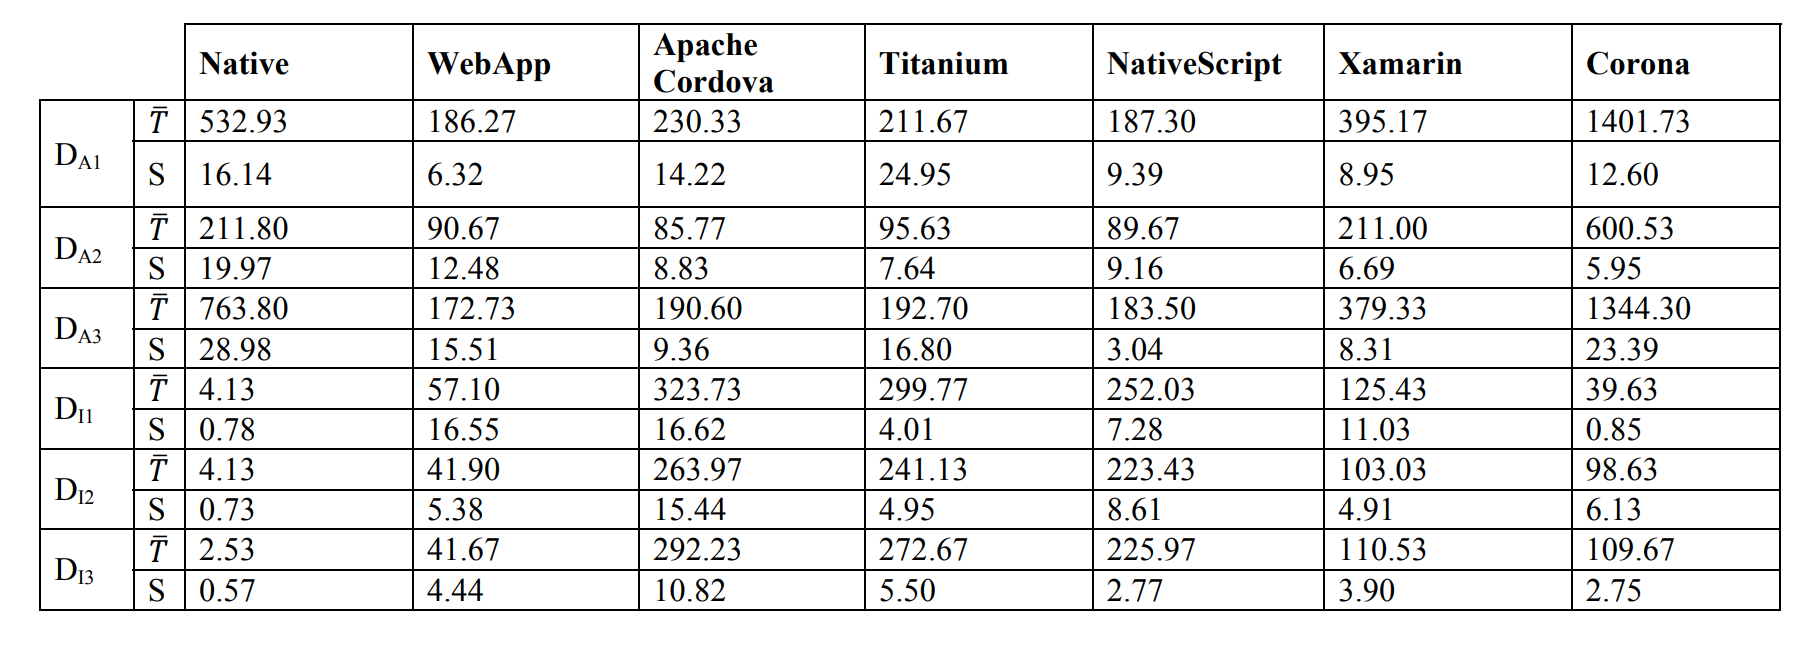
\includegraphics[width=\textwidth,keepaspectratio]{images/IEEE_Delia_Al.png}
  \caption[Ergebnisstabelle der Performancemessungen von Delia et al]{Ergebnisstabelle der Performancemessungen von Delia et al \cite{IEEE_development_classes}}
  \label{fig:result_table_IEEE_related_work}
\end{figure}

Einige Arbeiten drehen sich um den Faktor Performance. Delia et al \cite{IEEE_development_classes} etwa testet diese anhand von komplexen mathematischen Berechnungen und zeichnet dabei die verstrichene Zeit für iOS und Android auf. Dabei berechneten sie außerdem die Standardabweichung um zu untersuchen, wie gestreut die Ergebnisse sind. In Abbildung \ref{fig:result_table_IEEE_related_work} können diese betrachtet werden, dabei ist T die Zeit in ms die die Berechnung gedauert hat und S die Standardabweichung. Dabei ist ein möglichst kleiner Wert optimal. Sie stellte dabei einen Performance Unterschied zwischen Android und iOS fest, dieser ist jedoch ihrer Meinung nach, auf die unterschiedliche Hardware der Testgeräte zurückzuführen. Insgesamt stellte sie eine gute Performance von Web Applikationen fest. Die nativen Applikationen schnitten auf Android schlechter ab als ein Großteil der restlichen untersuchten Ansätze, auf iOS jedoch war dieser Ansatz der am besten performende.

In dieser Arbeit werden alle Tests auf einem Gerät durchgeführt um eine Vergleichbarkeit zu erlangen. Außerdem wird die Arbeit lediglich auf Android beschränkt, um auf die unterschiedlichen Ansätze und nicht auf die Unterschiede zwischen den Plattformen einzugehen.
 
Denko et al \cite{Denko_performance} vergleichen neben der verbrauchte Zeit für mathematische Berechnungen ebenfalls die Auslastung der Geräte während verschiedenen Aufgaben und die Appgröße der kompilierten Apps. Dabei konnten sie feststellen, dass je nach Aspekt, unterschiedliche Ansätze der am besten abschneidenden war. So war etwa bei der Ausführung von Algorithmen die Native Implementierung die schnellste, während bei der der Cross-Compilierte Ansatz die geringste Auslastung der CPU hatte. Sie kommen daher auf den Schluss, dass kein Ansatz in Sachen Performance der beste ist und deswegen eher andere Faktoren betrachtet werden müssen um eine fundierte Entscheidung zu treffen.

Einige Arbeiten vergleichen auch lediglich die Unterschiede zwischen zwei unterschiedlichen Ansätzen. So auch Andersson \cite{Andersson_2022}, der in seiner Arbeit die Performanceunterschiede zwischen einer nativ und einer mit Flutter geschriebenen Cross-Plattform Android App vergleicht. Dabei untersuchte er verschiedene Funktionalitäten, die in vielen Apps vorkommen. So etwa unendliche Listen oder auch Datenbankoperationen. Das Ergebnis seiner Arbeit ist, dass kein eindeutig besserer Ansatz identifiziert werden kann, da etwa Flutter schneller und Ressourcenschonender bei der Decodierung von Dateien ist, während Animationen auf der nativen Anwendung besser laufen. Er stellt dabei fest, dass der Cross-Plattform Ansatz insgesamt keine schlechtere Performance als die native Entwicklung aufzeigt.

Die Arbeiten von Andersson und Denko et al identifizierten die Performance als keinen eindeutigen Faktor um eine Wahl treffen zu können. Deswegen soll in dieser Arbeit weitere Faktoren in den Vergleich einbezogen werden.

\begin{figure}[ht]
  \centering
  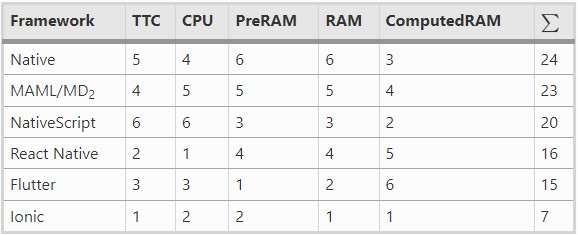
\includegraphics[width=10cm,keepaspectratio]{images/Biorn-Hansen_Result_table.jpg}
  \caption[Ergebnisstabelle der Untersuchung von Biørn-Hansen et al]{Ergebnisstabelle der Untersuchung von Biørn-Hansen et al \cite{BirnHansen.2020}}
  \label{fig:result_table_Biorn}
\end{figure}

Biørn-Hansen et al \cite{BirnHansen.2020} konzentrieren sich in ihrer Untersuchung vor allem auf die Nutzung Plattformspezifischer Schnittstellen, wie etwa der Geo-Daten oder Kontakte \ac{API}. Bei ihrer Auswertung der 5 Kriterien gewichten sie jeden, der 6 implementierten Ansätzen, anhand einer Zahl von 1 - 6, wobei 6 die Implementierung bekommt, die am besten in diesem Bereich abgeschlossen hat und 1, die die schlechtesten Ergebnisse lieferte. Danach werden die einzelnen erreichten Punkte zusammengerechnet. Wie in Abbildung \ref{fig:result_table_Biorn} zu sehen ist, erreichte Nativ dabei den 1. Platz mit einer Punktzahl von 24 Punkten. Das Cross-Plattform Framework Flutter hingegen landete auf dem vorletzten Platz mit gerade einmal 15 Punkten. In ihrem Fazit halten sie dementsprechend fest, dass die Nutzung von anderen Technologien zu einer Performanceverschlechterung führen kann, jedoch einige Frameworks in gewissen Bereichen besser abschneiden als die native Implementierung und es somit auf die genauen Anforderungen ankommt.

In ihrer Arbeit bewerten Biørn-Hansen et al die verschiedenen Ansätze anhand der gemessenen Werte. Dies führt dabei jedoch zu einer Verzerrung der Ergebnisse, da in einigen Kategorien die Unterschiede nur sehr gering waren, dies jedoch in ihrer Bewertung nicht berücksichtigt wird. Deswegen soll in der Arbeit von einer Gewichtung abgesehen werden und anhand von Kriterien Empfehlungen zu gewissen Technologien aufgeführt werden.

Raj und Tolety \cite{IEEE_Rahul_Seshu} stellen in ihrer Arbeit eine Einteilung von Applikationen in vier unterschiedliche Kategorien vor. Diese sind Applikationen,
\begin{itemize}
    \item die hauptsächlich eine Anzeige von Server Daten sind.
    \item die durch Nutzereingaben oder Sensoren Daten erhalten und diese verarbeiten,
    \item die ein eigenständiges System sind und keinerlei Verbindung zu einem Server oder anderen benötigen.
    \item die einen hohen Kommunikationsgrad mit einem Server haben.
\end{itemize}
Sie empfehlen, dass Entwickler den Entwicklungsansatz anhand der Appkategorie wählen. Beispielsweise empfehlen sie, dass bei viel Kommunikation mit einem Server, der Web-gestützte Ansatz gewählt wird. Sie sagen jedoch auch, dass Cross-Plattform Lösungen gut sind, wenn mehrere Plattformen abgedeckt werden sollen, da dadurch Entwicklungszeit und Kosten gespart werden können.

Ihre Erklärungen sind nachvollziehbar, jedoch fehlen in ihrer Arbeit Zahlen oder Entscheidungsfaktoren, um ihre Empfehlung zu stützen. Dazu wird in ihrer Auswertung die Klasse der Nativen Applikationen vernachlässigt. In dieser Arbeit soll deshalb anhand von konkreten Zahlen und Quellen ein Vergleich zwischen den implementierten Ansätzen gezogen werden, um eine nachvollziehbar Entscheidung zu stützen.

Olsson \cite{Olsson_2020} untersucht in ihrer Arbeit neben der Performance vor allem die Benutzeroberfläche und deren Benutzung. Dafür implementiert sie native Applikationen für iOS und Android und eine Cross-Plattform Flutter App, die auf beiden Plattformen installiert werden kann. Ihre Performancemessung zeigt, dass die Cross-Plattform Applikation eine gering schlechtere Performance als die nativen Implementierungen aufweist. Als zweiten Teil der Untersuchung befragt sie eine Gruppe an Entwicklern und zeigt ihnen in unterschiedlichen Anwendungsfällen der Android Implementierungen. Danach fragt sie nach Unterschieden und Auffälligkeiten zwischen den zwei anonymisierten Applikationen. Das Ergebnis ist, dass die Mehrheit der Befragten keinen Unterschied zwischen den zwei Anwendungen finden konnten. Der dritte Faktor ihrer Arbeit ist die Programmlänge, bei der die Cross-Plattform Implementierung die geringste Anzahl an Zeilen und benötigten Dateien hat. Insgesamt stellt sie fest, dass Flutter und damit Cross-Plattform Frameworks eine gute Alternative sein können, dies jedoch abhängig ist von der weiteren Entwicklung der Frameworks.

Die Arbeit von Olsson stellt eine umfangreiche Untersuchung zwischen den betrachteten Ansätzen dar. Jedoch ist die Arbeit lediglich auf zwei Ansätze beschränkt und bietet so nur einen guten Vergleich zwischen ihnen. Um mehr Aussagekraft über verschiedene Ansätze zu erhalten sollen deswegen in dieser Arbeiten mehr Ansätze untersucht werden. 

Khachouch et al \cite{IEEE_Khackouch_Al} erstellen in ihrer 2020 vorgestellten Arbeit einen Entscheidungsgraphen. Durch die Beantwortung einiger Fragen sollen Entwickler neuer Applikationen die für ihr Projekt passende Entwicklungsmethodik finden. Als erstes suchten sie dafür passende Fragen, die eine Eingrenzung erlauben und ordneten diesen ein Gewicht zu, um die Höhe der Frage in dem Graph festzulegen. Sie stellen am Ende fest, dass wenn es keine Einschränkungen in den Bereichen Entwicklungszeit und Kosten gibt, der native Ansatz aufgrund der besseren Performance und Qualität die beste Lösung bleibt. Durch ihren Graphen wird jedoch auch klar, dass oft andere Ansätze sinnvoller sein können.

Der von Kachouch et al vorgestellte Graph liefert innerhalb von 2 bis 8 Fragen eine eindeutige Antwort. In dieser Arbeit hingegen soll lediglich eine Tendenz aufgezeigt werden, da jedes Projekt durch seine einzelnen Funktionalität sehr komplex ist und nicht mit wenigen Fragen exakt eingeordnet werden kann. Stattdessen soll ein besseres Verständnis vermittelt werden, welche Faktoren eine Entscheidung beeinflussen können. 